\documentclass[12pt, titlepage]{article}
\documentclass{article}
\usepackage{graphicx}

\usepackage{booktabs}
\usepackage{tabularx}
\usepackage{hyperref}
\hypersetup{
    colorlinks,
    citecolor=black,
    filecolor=black,
    linkcolor=red,
    urlcolor=blue
}
\usepackage[round]{natbib}

%% Comments

\usepackage{color}

\newif\ifcomments\commentstrue

\ifcomments
\newcommand{\authornote}[3]{\textcolor{#1}{[#3 ---#2]}}
\newcommand{\todo}[1]{\textcolor{red}{[TODO: #1]}}
\else
\newcommand{\authornote}[3]{}
\newcommand{\todo}[1]{}
\fi

\newcommand{\wss}[1]{\authornote{blue}{SS}{#1}} 
\newcommand{\plt}[1]{\authornote{magenta}{TPLT}{#1}} %For explanation of the template
\newcommand{\an}[1]{\authornote{cyan}{Author}{#1}}

%% Common Parts

\newcommand{\progname}{Minimization Analysis} % PUT YOUR PROGRAM NAME HERE
\newcommand{\authname}{%Team \#, Team Name
%\\ Student 1 name
%\\ Student 2 name
%\\ Student 3 name
\\ Ning Wang} % AUTHOR NAMES                  

\usepackage{hyperref}
    \hypersetup{colorlinks=true, linkcolor=blue, citecolor=blue, filecolor=blue,
                urlcolor=blue, unicode=false}
    \urlstyle{same}
                                


\begin{document}

\title{Verification and Validation Report: \progname} 
\author{\authname}
\date{April 12, 2023}
	
\maketitle

\pagenumbering{roman}

\section{Revision History}

\begin{tabularx}{\textwidth}{p{3cm}p{2cm}X}
\toprule {\bf Date} & {\bf Version} & {\bf Notes}\\
\midrule
Apr 12 2023& 1.0 & First Draft\\
\bottomrule
\end{tabularx}

\newpage

\tableofcontents

\listoftables

%\listoffigures

\newpage

\section{Symbols, Abbreviations and Acronyms}

\renewcommand{\arraystretch}{1.2}
\begin{tabular}{l l} 
  \toprule		
  \textbf{symbol} & \textbf{description}\\
  \midrule 
  T & Test\\
  VnV & verification and validation\\
  \progname{} & Core Analysis\\
  \bottomrule
\end{tabular}\\
The complete table of symbols, abbreviations and acronyms can be found in the \href{https://github.com/KarenKarenWang/cas741_project1/blob/main/docs/SRS/SRS.pdf}{SRS} document of the software. 
\\


This document provides the information on validation and verification plans implemented for the \progname{} software. In this regard, the general approaches and plans are initially discussed and afterwards specific test cases and approaches for validation and verification of functional and nonfunctional requirements (can be found in \href{https://github.com/KarenKarenWang/cas741_project1/blob/main/docs/SRS/SRS.pdf}{SRS}) are reviewed. VnV plans here are a combination of manual (assigned to a member of the VnV team to assess) and automated testing approaches to evaluate the correctness of the information (whether input or output) or satisfaction of a goal in \progname{}. 

\pagenumbering{arabic}

\newpage
\section{Implementation Validation}
\subsection{Code Walkthrough}

This MATLAB program is designed to read data from a CSV file and optimize the power consumption and cost for a set of data centers using renewable and grid energy. The code reads information from the CSV file, extracts relevant data, sets up a linear programming optimization problem, and solves it using the linprog function. Here is a step-by-step walkthrough of the program:

\begin{itemize}
	\item Clear the workspace and command window.
	
	\item Request the user to input the CSV filename.
	\item Read the CSV file into a table using the readtable function.
	
\\	
        \item Extract the number of data centers {(num$_$data$_$centers)} and other relevant information such as distances, rates of renewable and grid energy, total and maximum power consumption from the table.
	
    \item Display the extracted information.
	
    \item Define constants and set up matrices for the linear programming optimization problem. The objective function 'f' is defined as a combination of renewable and grid energy costs. The constraint matrices A, b, Aeq, and beq are set up to represent the restrictions on power consumption from renewable and grid sources.
	
	
	
	\item Check for NaN values in the matrices. If any are found, display an error message and exit the program. 
	
	\item Solve the linear program using the linprog function.
	
	\item Check the solution exit flag. If the flag is not 1, display an error message and exit the program.
	
	\item Calculate the optimal power consumption for each data center from renewable and grid sources.
	

	
	\item Calculate the total cost of power consumption.
	
	\item Print the optimal power consumption and total cost for each data center.
	
	\item Plot the power consumption as a function of distance.
	
	
	
	\item Check if the constraints are satisfied. If not, print a message indicating that the constraints are not satisfied.
        \item Print the results for the current file and the total cost. If the constraints are satisfied, print "All constraints are satisfied." Otherwise, print "Constraints are not satisfied."

\end{itemize}
This program optimizes power consumption for a set of data centers, given the input data in a CSV file. It calculates the most cost-effective combination of renewable and grid energy to satisfy the power requirements while meeting the given constraints.
\\

\subsection{Functional Requirements Evaluation}
\label{func}
\paragraph{Test for R1:}

\begin{itemize}
    \item R1: Requirements for the inputs that are supplied by the user. This information has to be explicit.
    \item The program requests the user to input the CSV filename, which contains the necessary data for the optimization problem. The user should be provided with clear instructions on how to format the CSV file, including the required columns and their order.
\end{itemize}
\begin{figure}[h!]
\begin{center}
 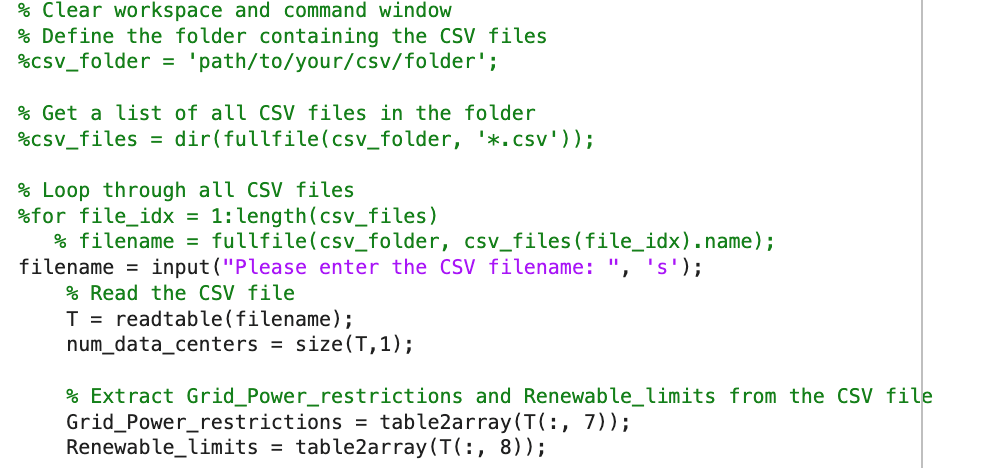
\includegraphics[width=0.6\textwidth]{for R1.png}
\caption{System Context}
\label{Fig_Proof for R1} 
\end{center}
\end{figure}
\paragraph{Test for R2:}

\begin{itemize}
    \item R2: The program shall notify the user if the input is out of bounds.


    \item The program checks for NaN values in the matrices but does not explicitly check for out-of-bound values in the input. Additional input validation should be implemented to notify the user if any input values are out of bounds.
\end{itemize}		 

\\
\paragraph{Test for R3:}

\begin{itemize}
    \item R3: User should keep input validate data type.
    \item The program reads data from the CSV file and directly converts it into the required data types (e.g., arrays, scalars). However, there is no explicit validation of data types in the input. Additional input validation should be implemented to ensure that the user-supplied data is of the correct data type.
\end{itemize}	

\\
\paragraph{Test for R4:}

\begin{itemize}
    \item R4: The program should be able to convert units while minimizing cost.
    \item The program currently minimizes the cost of power consumption based on the given rates for renewable and grid energy. It does not involve unit conversion. If unit conversion is required, the program should be updated to handle different units and perform the necessary conversions while minimizing cost.
\end{itemize}	

\\
\paragraph{Test for R5:}

\begin{itemize}
    \item R5: The program should keep all decision variables under their constraints.
    \item The program sets up the constraint matrices (A, b, Aeq, and beq) and solves the linear programming optimization problem. After solving the problem, it checks whether the constraints are satisfied within a specified tolerance. The program informs the user if the constraints are not satisfied.
\end{itemize}	


\paragraph{Test for R6:}

\begin{itemize}
    \item R6: The program output the optimal plan for end users.
    \item The program prints the optimal power consumption for each data center, both from renewable and grid sources, and the total cost. It also plots the power consumption as a function of distance. The output provides the user with an optimal plan for power consumption and cost.
\end{itemize}
\begin{figure}[h!]
\begin{center}
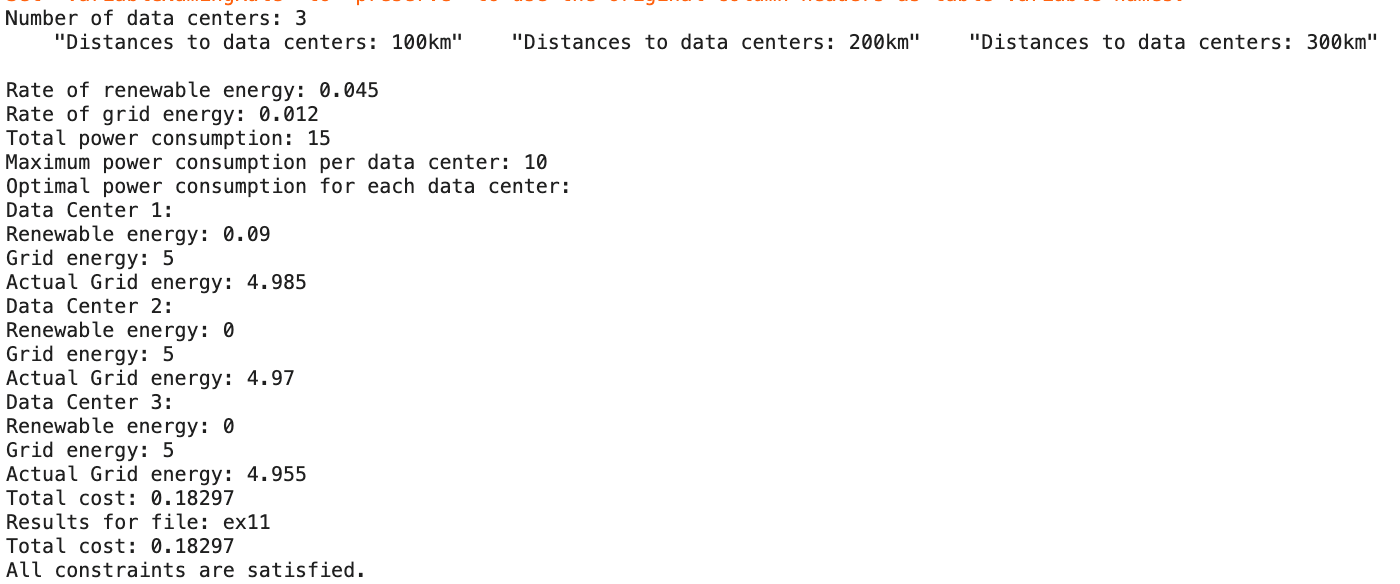
\includegraphics[width=0.6\textwidth]{for R6.png}
\caption{System Context}
\label{Fig_Proof for R6} 
\end{center}
\end{figure}


\paragraph{Test for R7:}

\begin{itemize}
    \item R7: The output should allocate the computing power of data centers with their capable size.


    \item The program optimizes power consumption based on the given constraints, such as maximum power consumption per data center. However, it does not explicitly allocate computing power. If allocation of computing power is required, the program should be updated to include this functionality.
\end{itemize}

\subsection{Tests for Nonfunctional Requirements}
\label{nonfunc}

\subsubsection{Test NFR1: Accuracy}
		
\paragraph{The accuracy of the computed solutions should meet the level needed for engineering application.}

\begin{itemize}
    \item The program uses the linprog function from MATLAB to solve the linear programming optimization problem, which is a well-established method for solving such problems. The accuracy of the computed solution should be sufficient for engineering applications. However, the user should validate the results and ensure the chosen tolerance level meets their specific requirements.
\end{itemize}


\subsubsection{Test NFR2: Usability}
		
\paragraph{The program shall not have a user interface but will clearly show the output, and data will be easy to copy and read.}

\begin{itemize}
    \item The program does not have a user interface, and it outputs the results in a clear and easy-to-read format. It prints the optimal power consumption and total cost for each data center and plots the power consumption as a function of distance. The user can easily copy the results and use them for further analysis.
\end{itemize}

\subsubsection{NFR3: Maintainability}
		
\paragraph{The time complexity of this program should be O(n).}

\begin{itemize}
    \item The program's time complexity is primarily determined by the linprog function, which has a time complexity that depends on the specific algorithm used and the problem size. Generally, the time complexity of linear programming solvers is higher than O(n). However, the program's overall complexity is dominated by the linear programming solver, and other operations in the program have relatively low time complexity.
\end{itemize}
\subsubsection{Test NFR4: Portability}
		
\paragraph{The program should be easily integrated with another software program.}

\begin{itemize}
    \item The program is written in MATLAB, which is widely used in engineering and scientific applications. It should be relatively easy to integrate the program with other MATLAB-based software. To integrate the program with software in other programming languages, the user may need to rewrite the program or use tools that enable communication between different programming languages (e.g., Python-MATLAB bridges or APIs).
\end{itemize}

\section{Unit Tests} \label{utest}

\subsection{Tests for Functional Requirements}

To run the unit test for this program, we'll refactor the program into 5 functions that can be individually tested. The detail of the unit test was illustrated in the command of code. The code can be found in \href{https://github.com/KarenKarenWang/cas741_project1/tree/main/docs/Design/code}{Code}

\subsubsection{Module 1: Test valid data}

\subsubsection{Module 2: Test invalid data}


\newpage

\section{Changes Due to Testing} \label{utest}
NA
\section{Automated Testing} \label{utest}
The program finally achieves automated and the Automated Testing code can be found in \href{https://github.com/KarenKarenWang/cas741_project1/tree/main/docs/Design/code}{Code}
 
\section{Trace to Requirements} \label{utest}
All requirements are satisfied in section 3.
\section{Trace to Modules} \label{utest}
All requirements are satisfied in section 4.
\newpage
\bibliographystyle{plainnat}

\bibliography{../../refs/References}

\end{document}